\begin{tcolorbox}[title={\Large Regularized Greedy Forest}]
	定期的に、全ての葉の重みを計算しなおすことで \\
	収束を早め、簡潔なモデルを作成する。 \\
	明示的な正則化があり、勾配ブースティングよりも調整しやすい。 \\
	決定木単位ではなく、葉ノード単位でアンサンブルを行う。 \\

	\begin{columns}
		\begin{column}{0.50\hsize}
			\[ F(x_i) = \sum_{v \in \mbox{\footnotesize leaves of }F} w_v r_v \]

			\vspace{50px}
			$r_0$ を $r_1$ と $r_2$ に分割した分類森 $F'$ は
			\begin{eqnarray*}
				F'
				&=& F - w_0 r_0 + w_1 r_1 + w_2 r_2  \\
				&=& F - w_0 r_0 + (w_0 + \delta_1) r_1 + (w_0 + \delta_1) r_2  \\
				&=& F + \delta_1 r_1 + \delta_2 r_2  \\
			\end{eqnarray*}

			\vspace{-70px}
			\[ \hat{\delta}_k = - \frac{Q'(F(\delta_1, \delta_2))}{Q''(F'(\delta_1, \delta_2))} \mid_{\delta_1=0, \delta_2=0} \]

		\end{column}
		\begin{column}{0.50\hsize}
			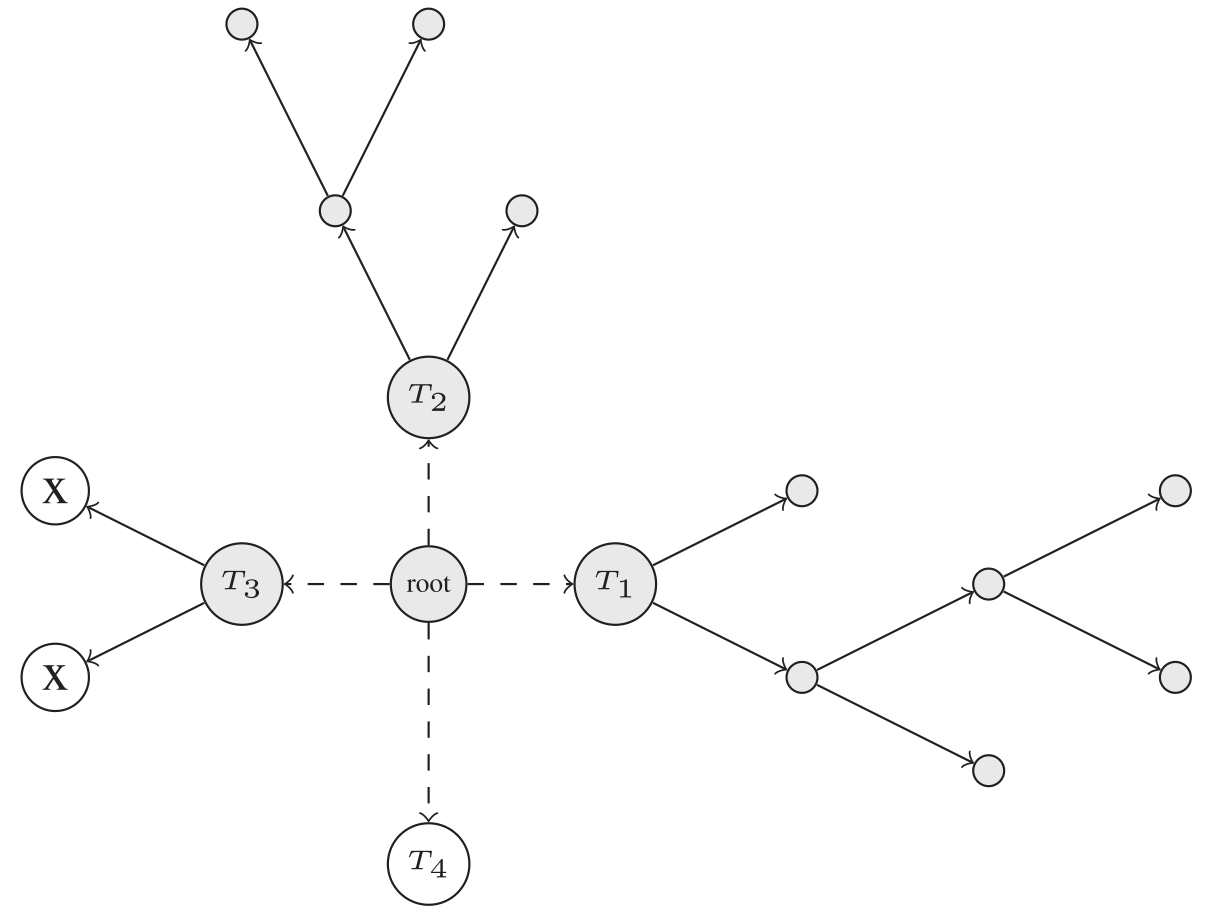
\includegraphics[width=1.0\textwidth]{img/rgf.png}
			\begin{textblock*}{\textwidth}(450pt,0pt)
				{\footnotesize 出典\cite{rgf}}
			\end{textblock*}
		\end{column}
	\end{columns}

	\vspace{40px}
	目的関数 $Q$ は
	\[
		\min Q
		= \sum^N_{i=1} \Phi(y_i, F(x_i)) + \Omega(F)
		= \sum^N_{i=1} \Phi(y_i, F(x_i)) + \lambda \sum_v w_v^2 / 2
	\]
	分割の目的は
	\begin{eqnarray*}
		\min Q' - Q
		&=& \Phi(y_i, w_1 r_1) + \Phi(y_i, w_2 r_2) - \Phi(y_i, w_0 r_0) + w_1^2 + w_2^2 - w_0^2 \\
		&=& \Phi(y_i, w_1 r_1) + \Phi(y_i, w_2 r_2) + w_1^2 + w_2^2 \\
	\end{eqnarray*}

\end{tcolorbox}
